\begin{frame}{some intuition (based on BBR)}
\small (based on Google's BBR presentation to the IETF) \\
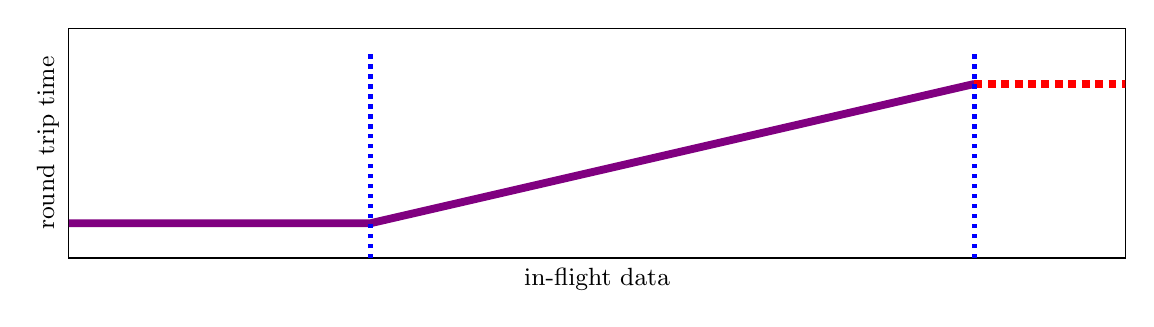
\begin{tikzpicture}
\begin{axis}[width=15cm,height=4.5cm,
    ylabel=round trip time,
    xlabel=in-flight data,
    label style={font=\small},
    tick label style={font=\small},
    ticks=none,
    xmin=0,xmax=35,ymin=0]
\addplot[violet,line width=1mm] coordinates {
(0, 1) (10, 1) (30, 5)
};
\addplot[red,dotted,line width=1mm] coordinates {
    (30, 5) (40, 5)
};
\addplot[blue,dotted,ultra thick] coordinates {
    (10, 0) (10, 6)
};
\addplot[blue,dotted,ultra thick] coordinates {
    (30, 0) (30, 6)
};
\end{axis}
\end{tikzpicture}
\vspace{-.5cm}
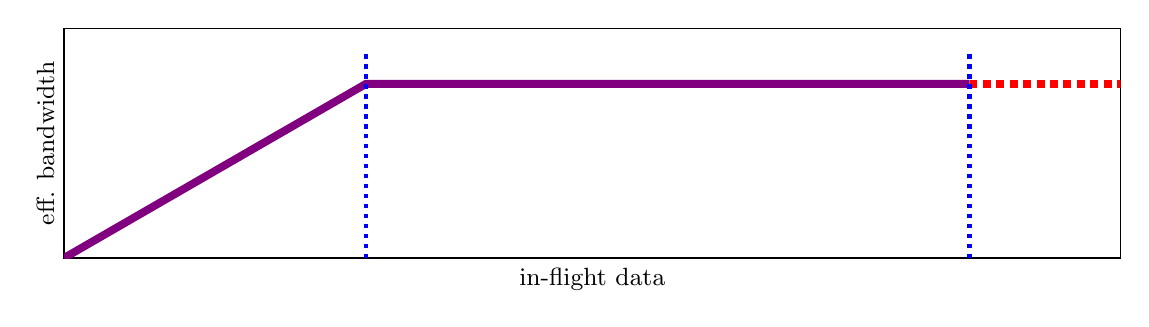
\begin{tikzpicture}
\begin{axis}[width=15cm,height=4.5cm,
    ylabel=eff. bandwidth,
    xlabel=in-flight data,
    label style={font=\small},
    tick label style={font=\small},
    ticks=none,
    xmin=0,xmax=35,ymin=0]
\addplot[violet,line width=1mm] coordinates {
(0, 0) (10, 5) (30, 5)
};
\addplot[red,dotted,line width=1mm] coordinates {
    (30, 5) (40, 5)
};
\addplot[blue,dotted,ultra thick] coordinates {
    (10, 0) (10, 6)
};
\addplot[blue,dotted,ultra thick] coordinates {
    (30, 0) (30, 6)
};
\end{axis}
\end{tikzpicture}
\end{frame}

\begin{frame}{very different congestion control}
    \begin{itemize}
    % FIXME: Fig 32 from TCPCC book
    \item fuller queues $\rightarrow$ higher latency
    \item fuller queues $\rightarrow$ throughput same as window increases
    \vspace{.5cm}
    \item<2-> strategy: monitor throughput/latency to detect full queues
        \begin{itemize}
        \item goal: fill link without making queue grow (much) in size
        \end{itemize}
    \end{itemize}
\end{frame}


\begin{frame}{`Vegas'-style congestion control (1)}
    \begin{itemize}
    \item record ``base'' round-trip time
        \begin{itemize}
        \item connection start or lowest observed
        \end{itemize}
    \item ``ideal'' throughput should be one window / base round trip time
        \begin{itemize}
        \item (Vegas paper calls this ``expected'' throughput)
        \item what would happen with no queuing delay
        \end{itemize}
    \item ``actual'' throughput $\approx$ one window / actual round trip time
    \end{itemize}
\end{frame}

\begin{frame}{`Vegas'-style congestion control (2)}
    \begin{itemize}
    \item measured ideal+actual throughput (prev. slide)
        \begin{itemize}
        \item mainly using idea of `base' round trip time
        \end{itemize}
    \vspace{.5cm}
    \item goal: control what ``ideal'' - actual throughput is
    \item if 0, queues are probably empty, can increase window
    \item if large, queues are too big, decrease window
    \end{itemize}
\end{frame}

\begin{frame}{Compound TCP}
    \begin{itemize}
    \item combines Vegas and `normal' TCP congestion control
    \item track seperate `delay' and `congestion' window
    \begin{itemize}
        \item congestion window uses standard TCP algorithm
        \item delay window based on Vegas-like increase in RTT detection
    \end{itemize}
    \item effective window size based delay+congestion window
    \vspace{.5cm}
    \item was default on Windows for many years
    \end{itemize}
\end{frame}

\begin{frame}{BBR-style congestion control}
    \begin{itemize}
    \item \myemph<2>{if queues are empty}, larger window:
    \item latency stays the same and throughput increases
    \vspace{.5cm}
    \item \myemph<3>{if queues are filling}, larger window:
    \item throughput stays the same and latency increases
    \vspace{.5cm}
    \item<4-> observe effect of sending more/fewer packets periodically
    \item<4-> estimate `boundary' based on observed latency/throughput
    \item<4-> keep window size near boundary most of the time
    \end{itemize}
\end{frame}

